\documentclass[aspectratio=169]{beamer}

\usepackage{ctex}
\usepackage{amsmath, amsfonts, amssymb, bm}
\usepackage{graphicx}
\usepackage{hyperref}
\usepackage{booktabs}
\usepackage{array}
\usepackage{tabularx}
\usepackage{ragged2e}

\graphicspath{{submission/baseline_study/figures/}{submission/selector_ablation/}}

\usetheme{Berlin}
\usecolortheme{whale}
\useinnertheme[shadow=true]{rounded}
\usefonttheme[onlymath]{serif}
\setbeamercovered{transparent}
\setbeamertemplate{navigation symbols}{}
\hypersetup{hidelinks}

\newcolumntype{Y}{>{\RaggedRight\arraybackslash}X}
\newcommand{\good}[1]{\textcolor{green!45!black}{#1}}
\newcommand{\warn}[1]{\textcolor{orange!80!black}{#1}}
\newcommand{\bad}[1]{\textcolor{red!70!black}{#1}}
\newcommand{\tightcaption}[1]{\vspace{0.5mm}{\scriptsize\color{black!70}#1}}

\setbeamertemplate{footline}{%
 \leavevmode%
 \hbox{%
 \begin{beamercolorbox}[wd=.31\paperwidth,ht=2.25ex,dp=1ex,center]{author in head/foot}
 平步青云
 \end{beamercolorbox}%
 \begin{beamercolorbox}[wd=.38\paperwidth,ht=2.25ex,dp=1ex,center]{title in head/foot}
 QBB-MIQP 5分钟路演
 \end{beamercolorbox}%
 \begin{beamercolorbox}[wd=.31\paperwidth,ht=2.25ex,dp=1ex,center]{date in head/foot}
 2026年5月17日 \quad \insertframenumber/\inserttotalframenumber
 \end{beamercolorbox}%
 }
}

\title[QBB-MIQP 路演]{QBB-MIQP：面向 MIQP 的量子-经典混合分解求解器}
\subtitle{不赌全局大线路，只打最关键的二进制块}
\author[平步青云]{混合整数优化问题赛道 · 平步青云}
\institute[Quantum MIQP]{Quantum Block-Benders for Mixed-Integer Quadratic Programming}
\date{2026年5月17日}

\begin{document}

\begin{frame}
 \titlepage
 \vspace{-5mm}
 \begin{alertblock}{5分钟先给结论}
 A/B 公开样例均达到官方最优；B 样例目标值 \textbf{610.266639}，gap \textbf{0\%}。核心不是把 MIQP 硬塞进大 QUBO，而是把量子/量子启发搜索限制在高价值 \textbf{20-bit block}，再用 LP 验真连续变量。
 \end{alertblock}
\end{frame}

\section{痛点}

\begin{frame}{痛点：直接 QUBO 化会把难点放大}
\small
\begin{columns}[T,onlytextwidth]
\begin{column}{0.32\textwidth}
\begin{block}{连续变量不能乱离散}
MIQP 中的 $y$ 若为进量子线路而离散化，精度越高，所需 qubit 越快爆炸。
\end{block}
\end{column}
\begin{column}{0.32\textwidth}
\begin{block}{二进制搜索空间巨大}
B 样例有 $n=80$ 个二进制变量，全局搜索空间为 $2^{80}$；全局 QAOA/枚举都不现实。
\end{block}
\end{column}
\begin{column}{0.32\textwidth}
\begin{block}{约束惩罚极不稳定}
惩罚项过小会不可行，过大又淹没原目标，量子层只是在追惩罚。
\end{block}
\end{column}
\end{columns}

\vspace{3mm}
\begin{alertblock}{真正问题}
关键不是“能不能写成 QUBO”，而是：\textbf{有限量子资源下，哪一小块二进制变量最值得搜索，并且搜索后如何保证真可行。}
\end{alertblock}
\end{frame}

\section{方法}

\begin{frame}{方案：QBB-MIQP 的混合闭环}
\small
\begin{columns}[T,onlytextwidth]
\begin{column}{0.58\textwidth}
\centering
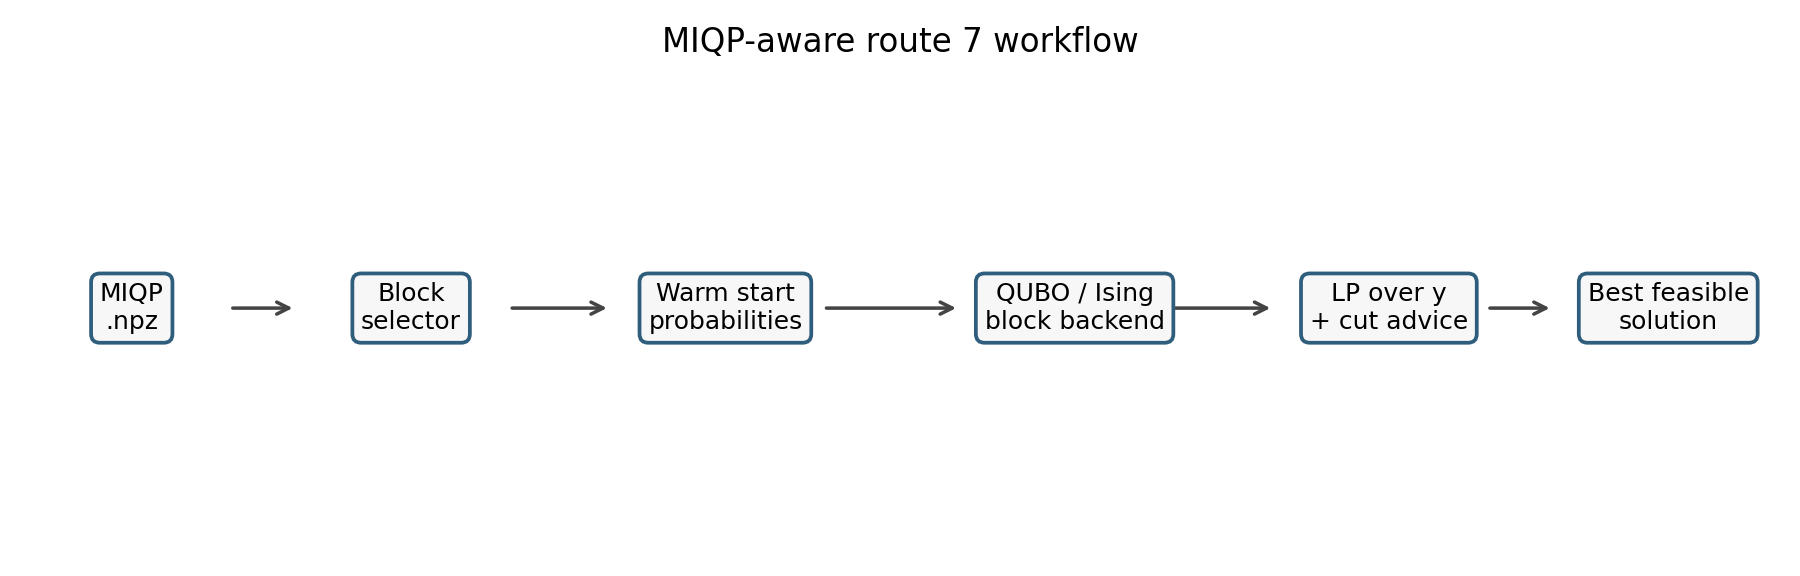
\includegraphics[width=\linewidth,height=0.60\textheight,keepaspectratio]{miqp_route7_workflow.png}
\tightcaption{论文图：QBB-MIQP 工作流。量子/启发式 backend 只处理高价值二进制 block。}
\end{column}
\begin{column}{0.39\textwidth}
\begin{block}{1. 分解}
固定 $x$ 后，连续 $y$ 子问题由 LP 精确求解，不把连续变量离散进线路。
\end{block}
\begin{block}{2. 搜索}
根据 $Q,A,B,G$ 结构、warm start 和历史改进选择关键 block，交给 exact / annealing / learning-guided / QAOA-compatible backend。
\end{block}
\begin{alertblock}{3. 验真}
候选必须经过 repair + LP，再用原始 MIQP 目标值与约束报告排序。
\end{alertblock}
\end{column}
\end{columns}
\end{frame}

\begin{frame}{为什么能赢：分块质量决定上限}
\scriptsize
\begin{columns}[T,onlytextwidth]
\begin{column}{0.48\textwidth}
\centering
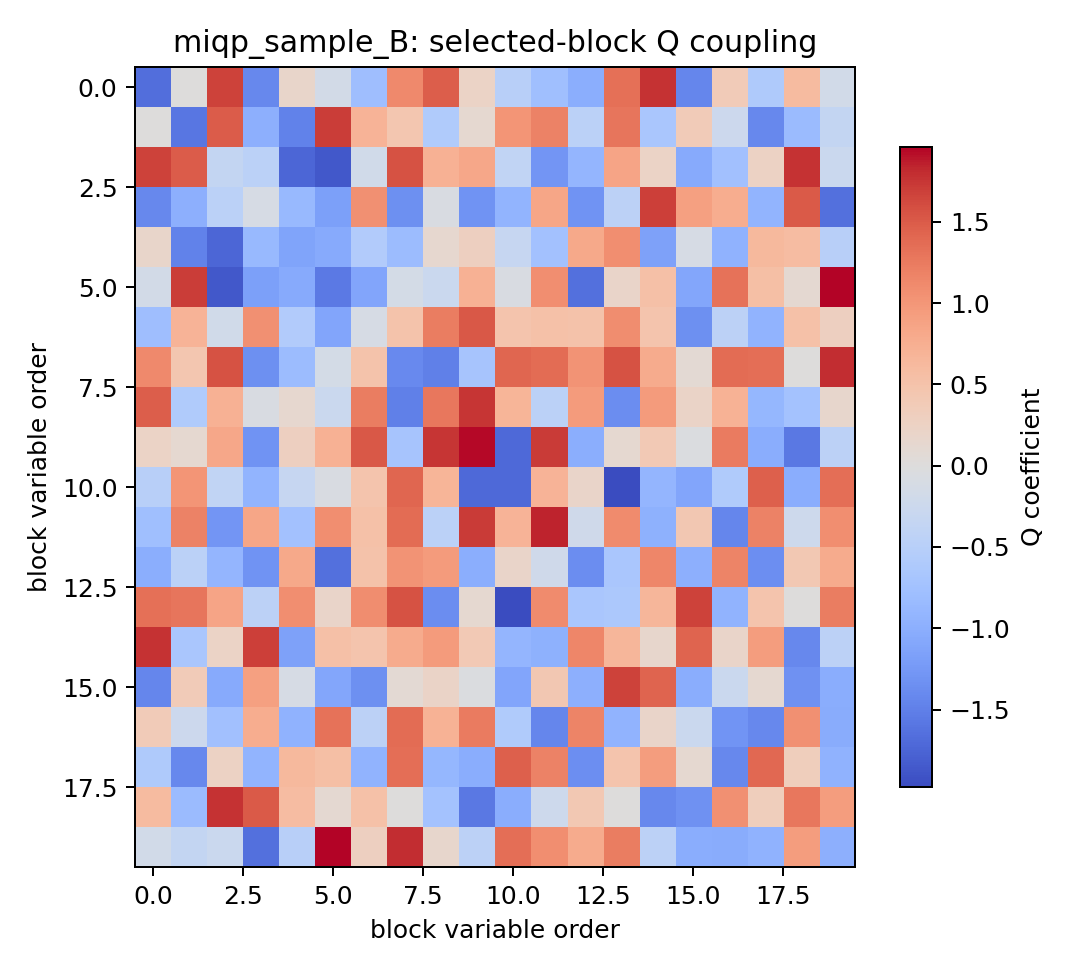
\includegraphics[width=\linewidth,height=0.47\textheight,keepaspectratio]{miqp_sample_B_block_coupling_heatmap.png}
\tightcaption{论文图：B 样例二进制变量耦合热图。强耦合变量需要被一起搜索。}
\end{column}
\begin{column}{0.48\textwidth}
\centering
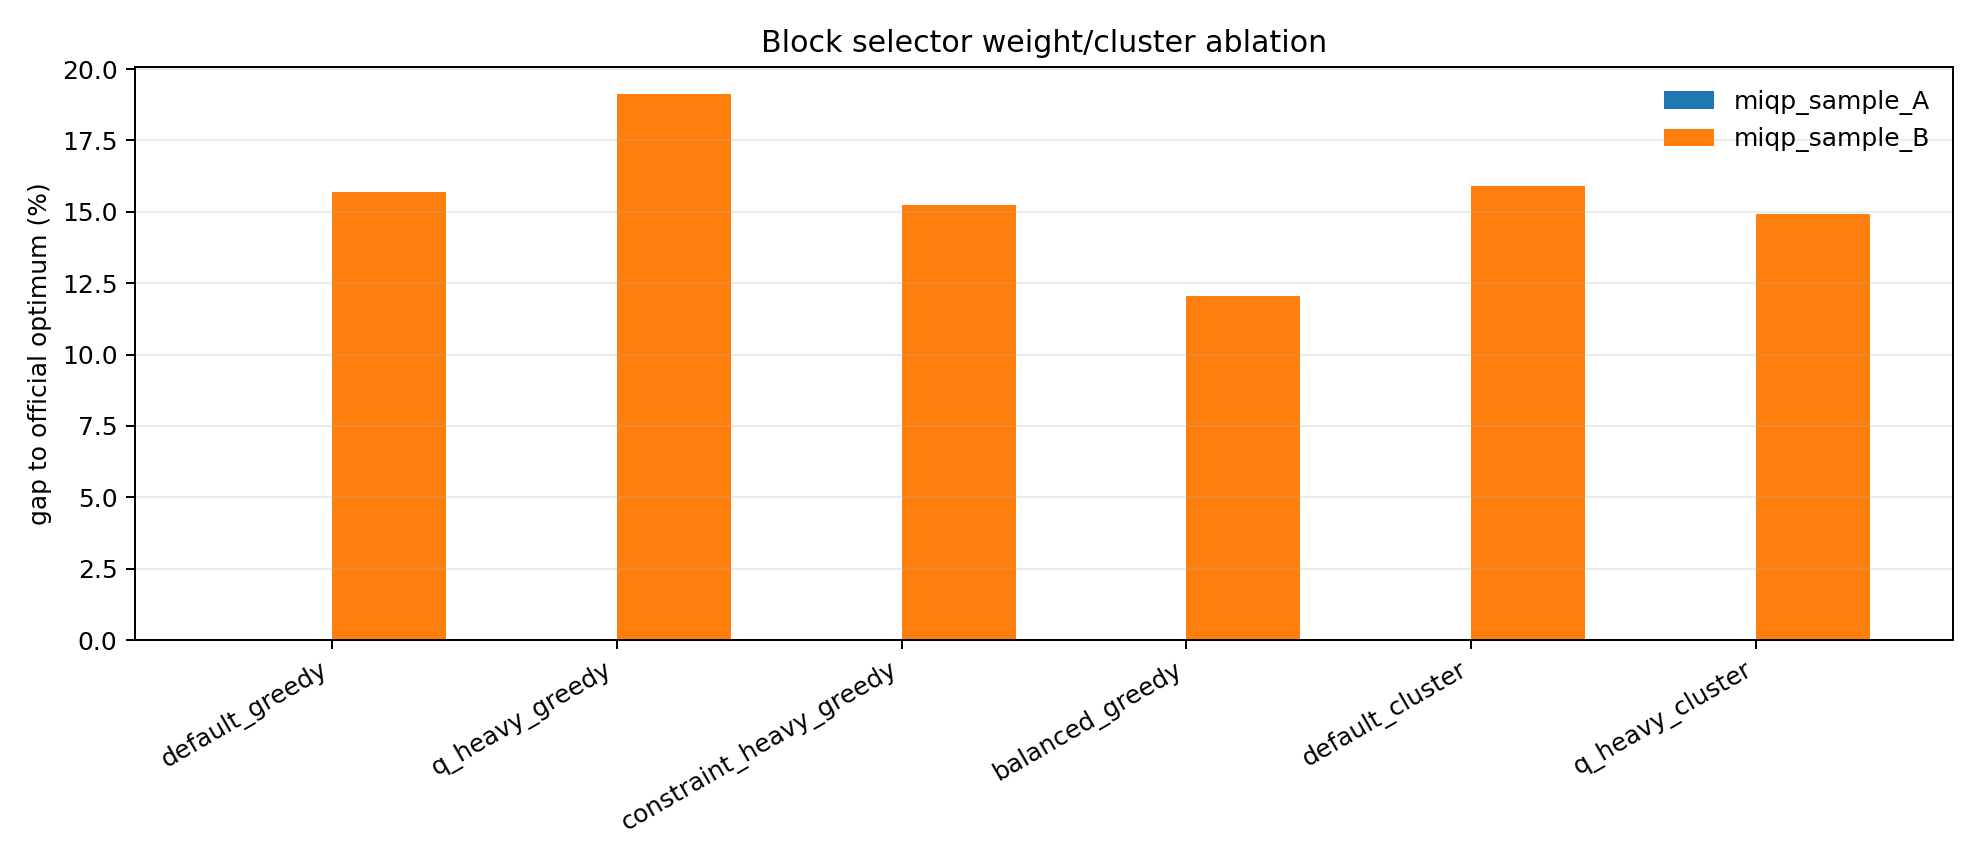
\includegraphics[width=\linewidth,height=0.47\textheight,keepaspectratio]{selector_ablation_gap.png}
\tightcaption{论文图：selector 消融。简单切块在 B 上仍留下显著 gap。}
\end{column}
\end{columns}

\vspace{2mm}
\begin{block}{QBB-MIQP 的判断}
不是“随机切 20 bit”，而是用目标耦合、混合约束参与度、选择约束压力、warm-start probability 和 cut advice 共同决定 block pool。
\end{block}
\end{frame}

\section{结果}

\begin{frame}{结果证据：A/B 达到官方最优}
\scriptsize
\begin{columns}[T,onlytextwidth]
\begin{column}{0.47\textwidth}
\centering
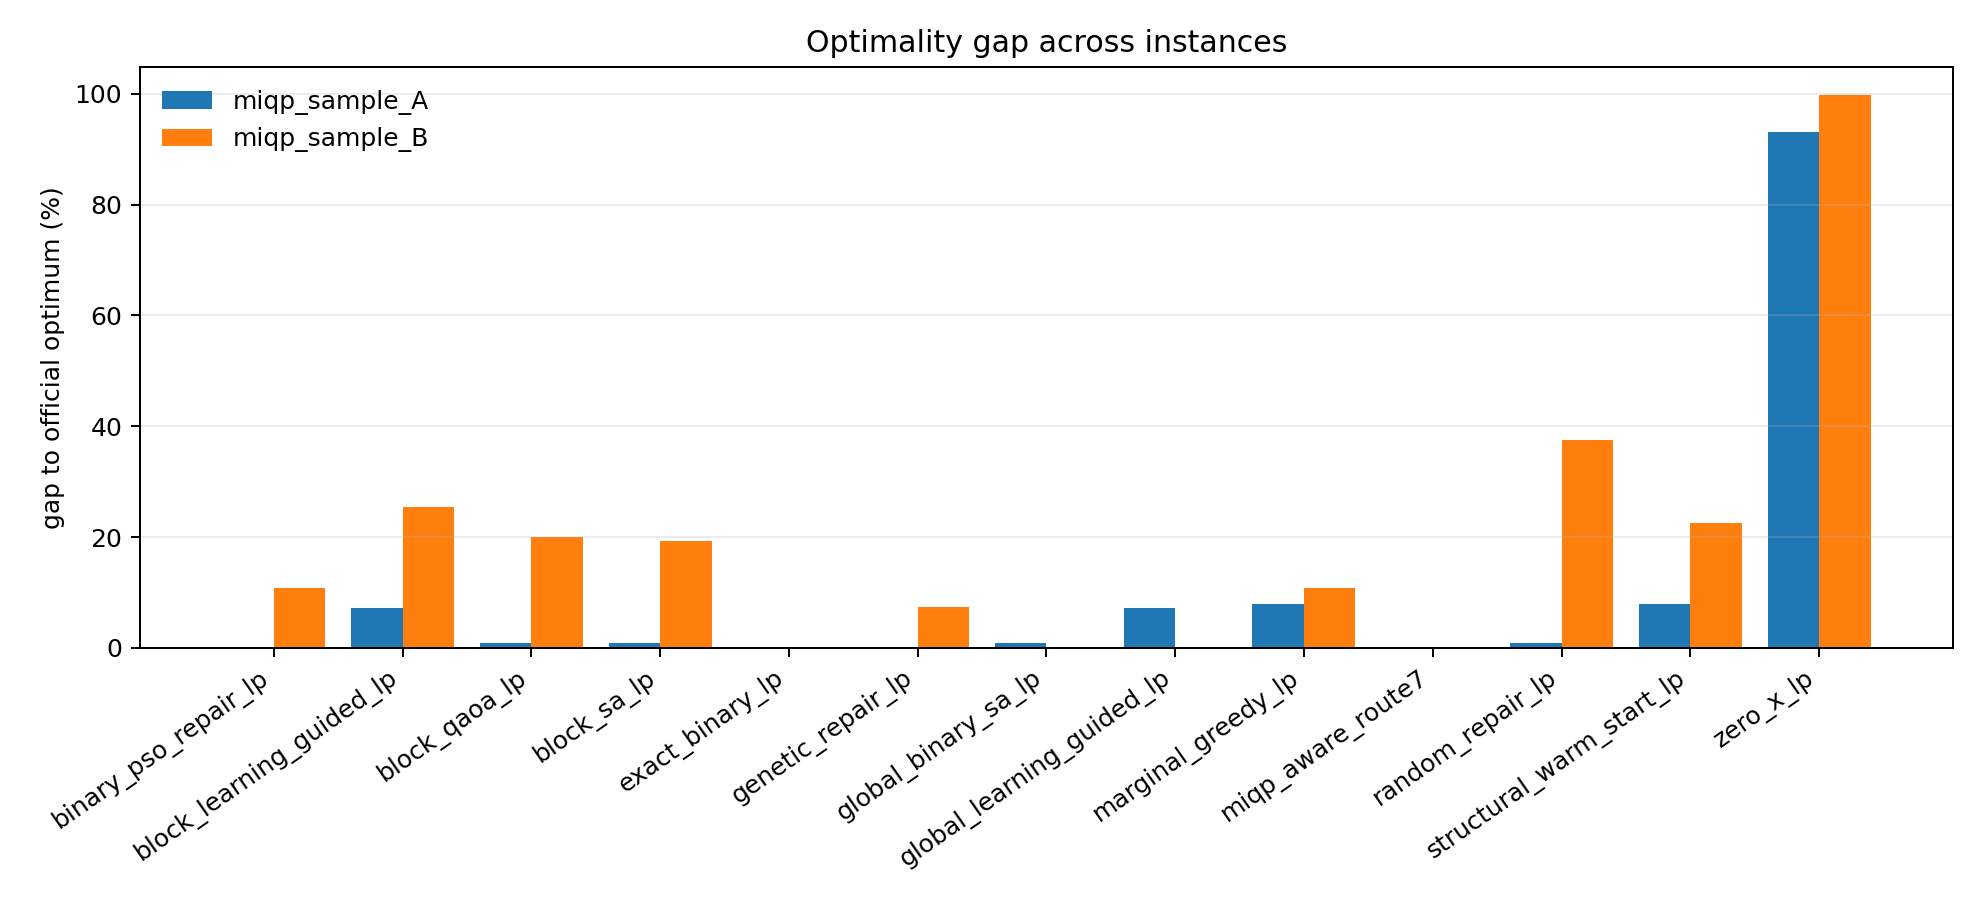
\includegraphics[width=\linewidth,height=0.43\textheight,keepaspectratio]{cross_instance_gap.png}
\tightcaption{论文图：跨样例 gap 对比。QBB-MIQP 在 A/B 均为 0\%。}
\end{column}
\begin{column}{0.50\textwidth}
\centering
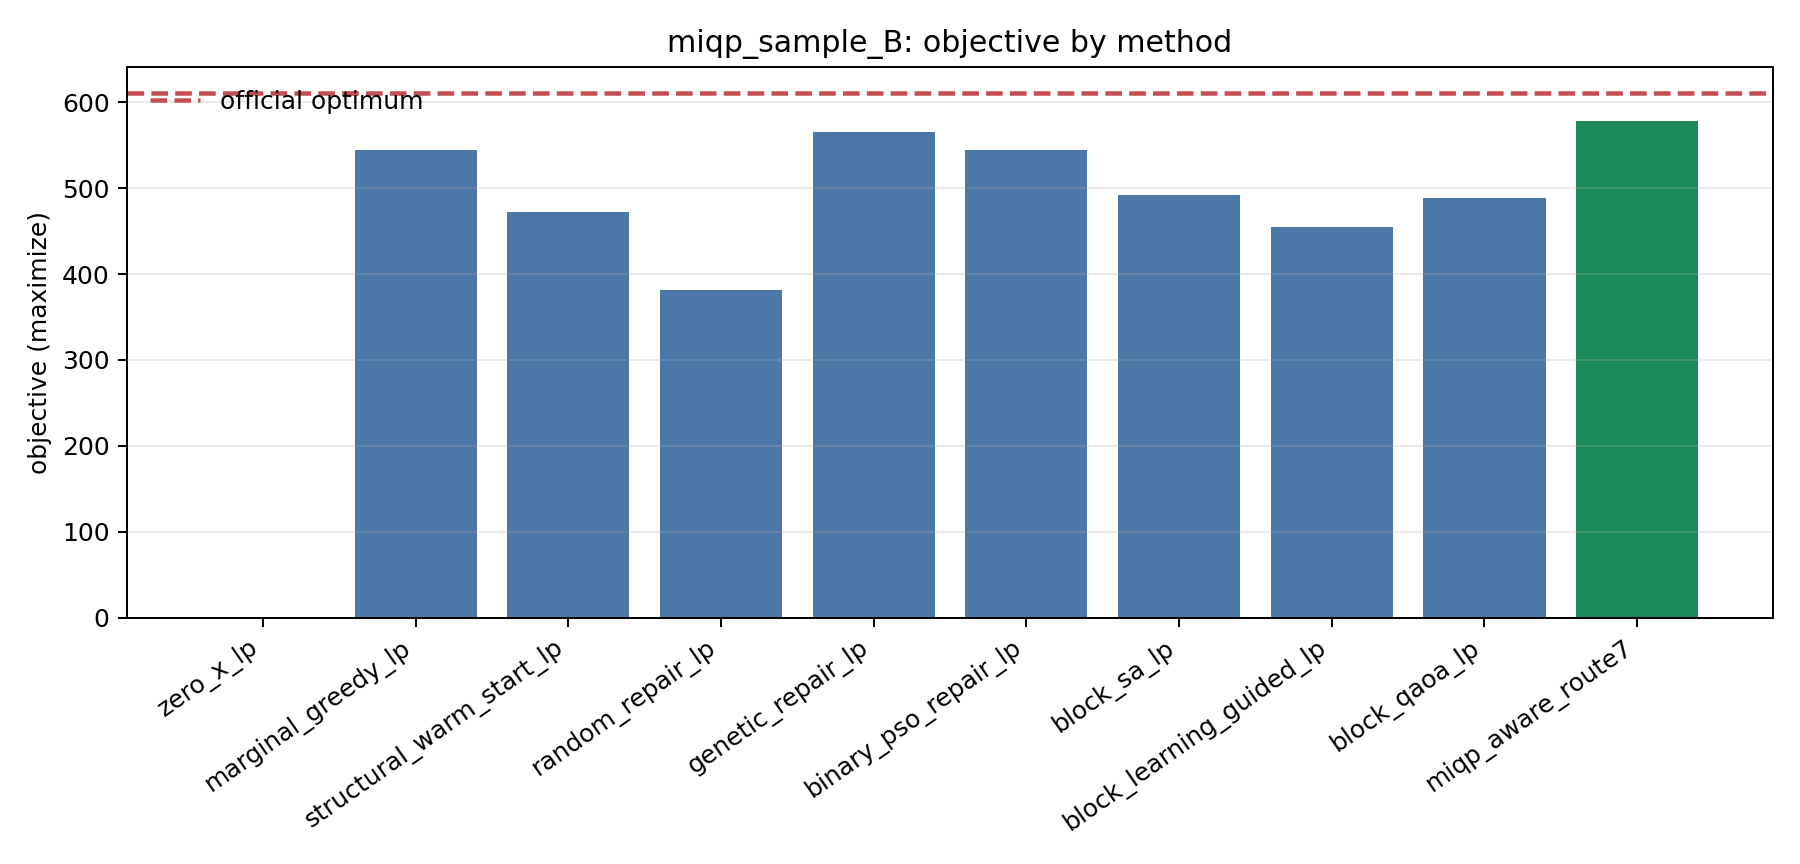
\includegraphics[width=\linewidth,height=0.43\textheight,keepaspectratio]{miqp_sample_B_objective_by_method.png}
\tightcaption{论文图：B 样例目标值横向对比。}
\end{column}
\end{columns}

\vspace{1mm}
\begin{alertblock}{B 样例核心数字}
\centering
\begin{tabular}{lcccc}
\toprule
方法 & 目标值$\uparrow$ & Gap$\downarrow$ & 候选验证 & 备注 \\
\midrule
GA + repair & 565.761894 & 7.29\% & 146 & 强经典基线 \\
Block-QAOA + LP & 488.070768 & 20.02\% & 146 & 10-qubit 量子基线 \\
\textbf{QBB-MIQP} & \textbf{610.266639} & \textbf{0.00\%} & \textbf{768} & \textbf{官方最优} \\
\bottomrule
\end{tabular}
\end{alertblock}
\end{frame}

\begin{frame}{复现与交付：明天数据来了，直接跑}
\scriptsize
\begin{columns}[T,onlytextwidth]
\begin{column}{0.50\textwidth}
\centering

\includegraphics[width=\linewidth,height=0.47\textheight,keepaspectratio]{miqp_sample_B_resource_profile.png}
\tightcaption{论文图：资源画像。block 搜索，而非全局 80-qubit。}
\end{column}
\begin{column}{0.47\textwidth}
\begin{block}{工程复现与入口}
堡垒机 \texttt{qiskit} 容器已完成源码包解压、安装、测试与 A/B 重跑。隐藏测试入口：\texttt{scripts/run\_miqp\_hidden\_demo.py}。
\end{block}
\vspace{-1mm}
\begin{alertblock}{隐藏测试预案}
\begin{itemize}
  \item test 1：exact-QUBO + LP。
  \item test 2--3：subQUBO / block pool。
  \item test 4--5：cluster/cut-guided + portfolio stress。
\end{itemize}
\centering
\textbf{不赌全局大线路；只打最关键的二进制块。}
\end{alertblock}
\end{column}
\end{columns}
\end{frame}

\end{document}
